%*==================================================================================*
% *                     Review vs. Camera-Ready settings                             *
% *==================================================================================*
%
% REVIEW: Use the following command for submitting the paper (double-blind,
% for review):
\documentclass{Interspeech}
%
% CAMERA-READY: Use the following command for the camera-ready version, one
% affiliation per line:
% \documentclass[cameraready]{Interspeech}
% *==================================================================================*

\usepackage{cite}
\usepackage{multirow}

% **************************************
% *                                    *
% *      STOP !   DO NOT DELETE !      *
% *          READ THIS FIRST           *
% *                                    *
% * This template also includes        *
% * important INSTRUCTIONS that you    *
% * must follow when preparing your    *
% * paper. Read it BEFORE replacing    *
% * the content with your own work.    *
% **************************************

%==================================================================================
% Title
% Must exactly match the title entered into the paper submission system
\title{DramaPara: A TV Drama Dataset for Enhancing Paralinguistic Understanding in Large Audio-Language Models}

%==================================================================================
% Authors
% The order of authors here must exactly match the order entered into the paper submission system
% Note that the COMPLETE list of authors MUST be entered into the paper submission system at the outset, including when submitting your manuscript for double-blind review
% The ORCID number is still optional but will become mandatory in the future years. It is strongly encouraged to get an ORCID for each cu-author.
% Middle names, including initials, must be included in the first name
\author[affiliation={1}, orcid=0000-0000-0000-0000, equalcontribution]{FirstNameA}{LastNameA}
\author[affiliation={2,3}, orcid=0000-0000-0000-1111, equalcontribution, correspondingauthor]{FirstNameB InitialB}{LastNameB}
\author[affiliation={1,3}]{FirstNameC}{LastNameC}
% The maximum number of authors in the author list is 20. If the number of contributing authors is more than this, they should be listed in a footnote or the acknowledgement section.

%==================================================================================
% Affiliations

\address{
    $^1$ Address Affiliation 1, Country Affiliation 1 \\
    $^2$ Address Affiliation 2, Country Affiliation 2 \\
    $^3$ Address Affiliation 3, Country Affiliation 3
}

%==================================================================================
% Emails
\email{first@university.edu, second@companyA.com, third@companyB.ai}

%==================================================================================
% Keywords
\keywords{paralinguistic understanding, large audio-language models, speech dataset}

\newcommand{\blue}[1]{\textcolor{blue}{#1}}
\newcommand{\red}[1]{\textcolor{red}{#1}}
\usepackage{comment}

%==================================================================================
% Content

\begin{document}

\maketitle

% the abstract here must exactly match the abstract entered into the paper submission system
\begin{abstract}
% While Large Audio Models (LAMs) have demonstrated remarkable versatility in speech processing, accurately parsing rich paralinguistic information—such as emotion, intonation, and speaking rate—in acoustically complex environments remains a significant challenge. This limitation stems primarily from a domain gap: existing paralinguistic datasets predominantly rely on idealized clean speech or studio-recorded voice acting, which deviate sharply from real-world acoustic diversity. To bridge this gap, we introduce \textbf{DramaPara}, a comprehensive TV drama dataset designed to enhance paralinguistic understanding in LAMs. Extracted from massive TV drama videos, DramaPara captures highly expressive human emotions and naturalistic background sound effects, maximizing the restoration of complex acoustic scenarios. The dataset is built through an efficient pipeline of LAM pre-annotation and fine-grained human calibration, featuring two core task paradigms: single-utterance isolated description ($\sim$492 hours) and multi-utterance sequential description ($\sim$213 hours) for capturing dynamic emotional evolution. To validate its efficacy, we apply a mixed training strategy incorporating Supervised Fine-Tuning (SFT) and Reinforcement Learning (RL) to open-source LAMs using DramaPara. Experimental results demonstrate that our approach yields a substantial 30.93\% average relative improvement in paralinguistic perception and description capabilities under complex scenarios, providing a high-quality data foundation for robust general audio understanding.
Large audio-language models (LAMs) struggle to parse paralinguistics (e.g., emotion, intonation) in acoustically complex environments. This stems from a domain gap: current datasets rely heavily on clean speech or studio recordings, lacking real-world diversity. To bridge this, we introduce DramaPara, a TV drama dataset designed to enhance LAMs' paralinguistic understanding. Extracted from TV shows, it features expressive human emotions and naturalistic background effects to mirror complex acoustic scenarios. Constructed via LAM pre-annotation and rigorous human calibration, DramaPara includes two tasks: single-utterance isolated description ($\sim$492h) and multi-utterance sequential description ($\sim$213h) to capture dynamic evolution. By applying a mixed training strategy (SFT and RL) on open-source LAMs, we demonstrate a 30.93\% average relative improvement in paralinguistic perception under complex scenarios, providing a vital data foundation for robust audio understanding.
\end{abstract}



\section{Introduction}
\label{sec:intro}

\begin{figure}[t]
  \centering
  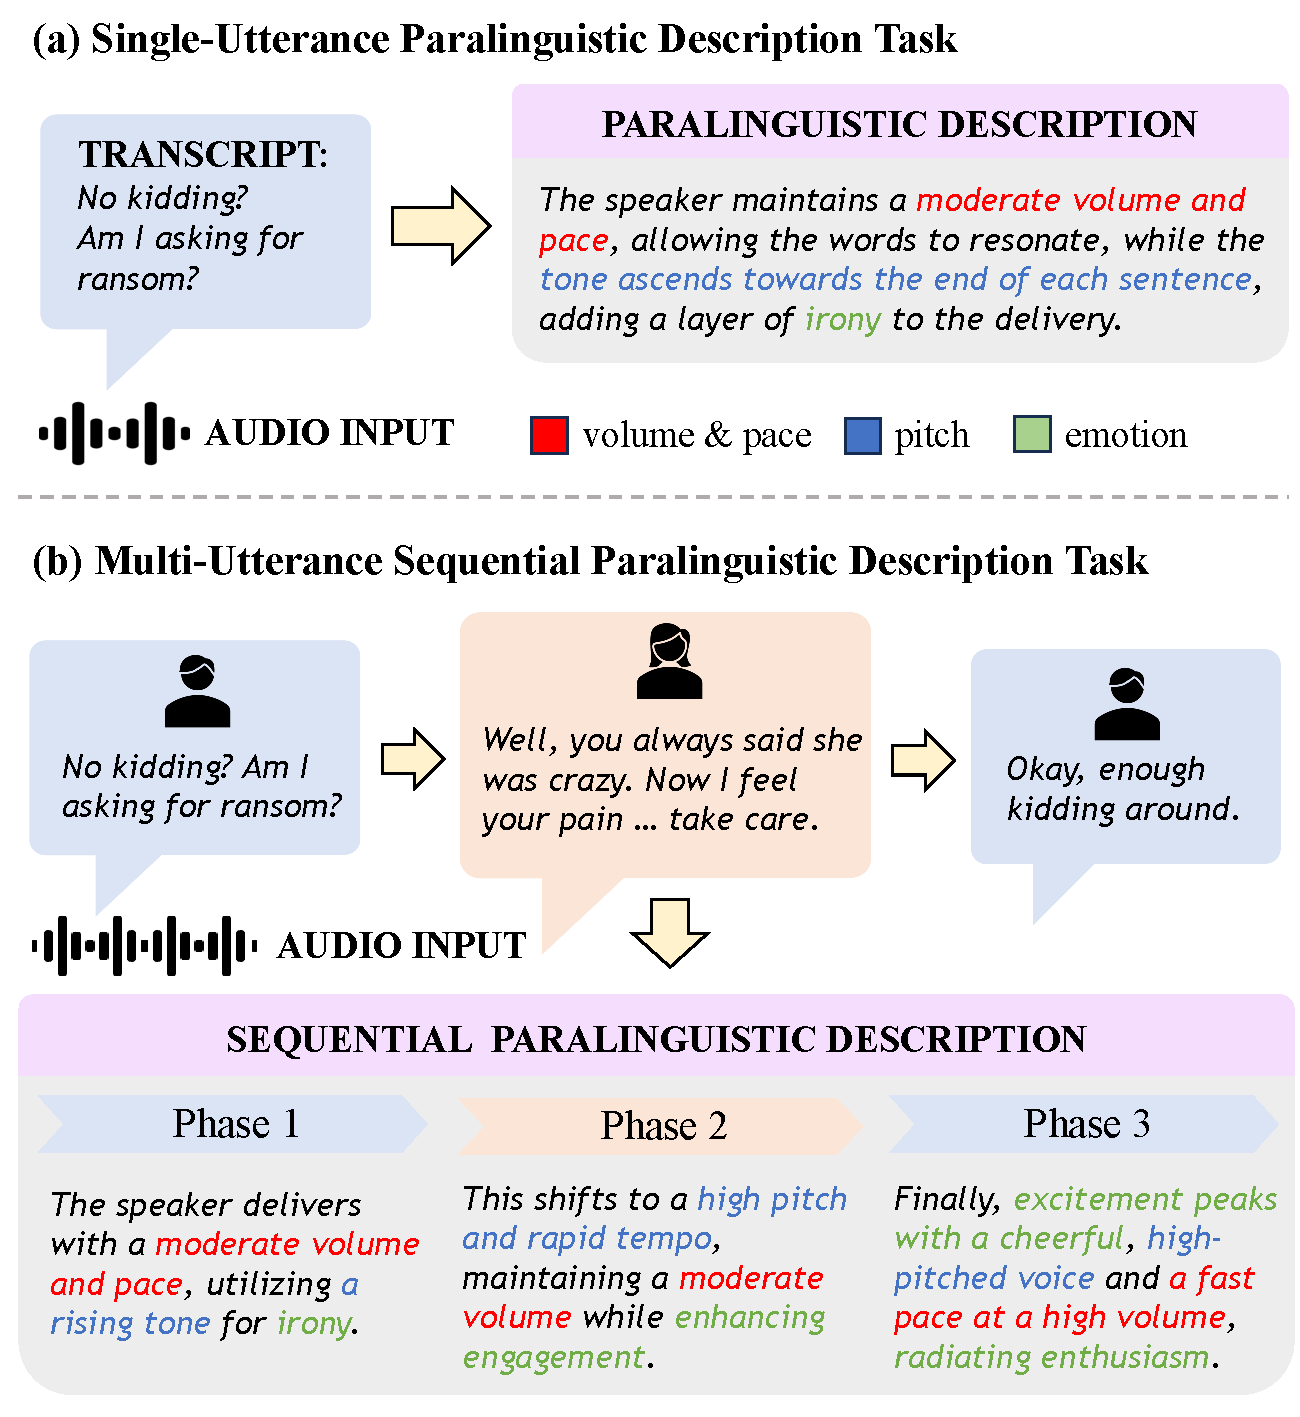
\includegraphics[width=\linewidth]{figs/task_fig.pdf}
  \caption{Overview of the two core task paradigms in the DramaPara dataset. (a) The Single-Utterance Paralinguistic Description Task generates a detailed textual profile for an isolated speech clip, explicitly capturing attributes such as volume, pace, pitch, and emotion. (b) The Multi-Utterance Sequential Paralinguistic Description Task processes continuous conversational turns to track chronological shifts, mapping the dynamic evolution of the speaker's paralinguistic state across different phases (e.g., transitioning from irony to excitement).}
  \label{fig:task_overview}
\vspace{-0.5cm}
\end{figure}

Human speech contains rich paralinguistic information, such as age, gender, emotional state, intonation, speaking rate, and volume. 
% In voice-based Human-Computer Interaction (HCI) systems, beyond accurately recognizing semantic content, deeply understanding and parsing this paralinguistic information is crucial for building natural, empathetic, and high-quality interactive experiences~\cite{dummy_citation_hci}.
% Traditional deep learning models are typically designed for single paralinguistic features (e.g., emotion recognition or gender classification)~\cite{dummy_citation_trad}. These models struggle with general paralinguistic understanding tasks, and their generalization capabilities are severely limited by the closed-set categories predefined during training. 
Recently, large audio-language models (LAMs) have demonstrated remarkable generalizability and versatility, capable of directly describing paralinguistic information in speech using natural language text~\cite{tangsalmonn, chu2023qwen, gong2023joint, hu2024wavllm, hurst2024gpt, chu2024qwen2, zeng2024glm, ding2025kimi, huang2025step, wu2025step}. However, when confronted with acoustically complex scenarios containing background noise, various sound effects, or intense, dynamic, blurry or complicated emotions, the perception and description capabilities of existing LAMs often lack accuracy and fine granularity.

The core reason for this limitation lies in the domain gap of the training data. Existing paralinguistic datasets are mostly built upon clean speech like LibriTTS~\cite{zen19_interspeech} and Emilia~\cite{Emilia}, or rely on Text-to-Speech (TTS) synthesis and studio-recorded voice acting~\cite{guo2023prompttts, busso2025msp, busso2008iemocap, lu24c_interspeech, SynParaSpeech, Zh_Paral, nagraniy2017voxceleb, nguyen23_interspeech, richter24_interspeech, TextrolSpeech, MM_TTS, SpeechCraft, kawamura24_interspeech, COCO_NUT, diwan-etal-2025-scaling, borisov25_ssw, NVSpeech}. These highly idealized clean audio recordings significantly deviate from real-world application scenarios characterized by complex and variable acoustic environments. Therefore, there is an urgent need to construct a high-quality, highly expressive paralinguistic fine-tuning dataset to further break through the understanding bottleneck of LAMs in open environments.

To address these challenges, we construct \textbf{DramaPara}, a comprehensive paralinguistic information understanding dataset tailored for naturalistic and complex scenarios. Specifically, we extract audio clips containing actor dialogues and complex background sound effects from massive TV drama videos, thereby closely approximating real-world acoustic environments and highly expressive human emotions. Regarding data annotation, we design an efficient pipeline comprising automatic pre-annotation by LAMs combined with fine-grained human calibration, ensuring the high quality and accuracy of the labels. To meet diverse interaction needs, we design two core task paradigms (as shown in Figure~\ref{fig:task_overview}): 1) \textbf{Single-utterance paralinguistic description} ($\sim$492 hours), focusing on the fine-grained profiling of the current isolated speech clip; 2) \textbf{Multi-utterance sequential paralinguistic description} ($\sim$213 hours), emphasizing the chronological capture of dynamic paralinguistic evolution in conjunction with context. Based on this dataset, we apply a mixed training strategy, incorporating Supervised Fine-Tuning (SFT) and Reinforcement Learning (RL), to existing open-source LAMs. Experimental results demonstrate that the fine-tuned models achieve a significant average relative improvement of 30.93\% in paralinguistic understanding and description capabilities in complex scenarios.

The main contributions of this work are summarized as follows:
\begin{itemize}
    \item We construct \textbf{DramaPara}, a novel paralinguistic dataset specifically designed for acoustically complex environments, comprising both single-utterance and multi-utterance sequential tasks. The entire dataset is strictly human-calibrated, effectively bridging the domain gap between existing clean datasets and real-world applications.
    \item We validate the capability-enhancing effect of the proposed dataset. Extensive experiments demonstrate that fine-tuning open-source LAMs (via SFT and RL) on \textbf{DramaPara} significantly enhances their paralinguistic understanding and description in complex acoustic environments, providing a high-quality data foundation for future general audio understanding research.
\end{itemize}

\section{Related Work}
\label{sec:related}

The development of robust speech language models heavily relies on high-quality paralinguistic datasets. However, existing corpora typically suffer from a domain gap compared to real-world acoustic environments. Based on their data curation paradigms, we broadly categorize them into two main groups.

\textbf{Self-Recorded and Studio-Collected Corpora:} Many foundational datasets are recorded from scratch in highly controlled environments to ensure acoustic purity. For instance, Expresso~\cite{nguyen23_interspeech}, MEAD~\cite{MM_TTS}, and Ears~\cite{richter24_interspeech} were strictly collected in professional recording studios or anechoic chambers. While corpora like VoxCeleb~\cite{nagraniy2017voxceleb} and the MSP-Podcast~\cite{busso2025msp} capture more naturalistic human voices, they still predominantly feature clean foreground speech with minimal acoustic interference. Consequently, these datasets inherently lack the complex background noises and intense, dynamic emotional fluctuations found in unconstrained scenarios.

\textbf{Aggregated and Synthesized Public Data:} To efficiently scale up data volume and diversity, a prevalent approach involves aggregating and processing existing datasets—ranging from the aforementioned studio-recorded corpora to larger-scale collections like LibriTTS and Emilia. DeSTA~\cite{lu24c_interspeech}, TextrolSpeech~\cite{TextrolSpeech}, SpeechCraft~\cite{SpeechCraft}, LibriTTS-P~\cite{kawamura24_interspeech}, ParaSpeechCaps~\cite{diwan-etal-2025-scaling}, and NonverbalTTS~\cite{borisov25_ssw} construct new datasets by combining these various public corpora and appending attribute metadata. Other efforts, such as PromptSpeech~\cite{guo2023prompttts}, rely heavily on TTS models to artificially synthesize paralinguistic features. Consequently, these aggregated datasets often inherit the idealized acoustic properties of their sources or introduce synthetic artifacts, restricting their generalizability in diverse scenarios.

% \textbf{Advantages of DramaPara:} In stark contrast to the clean audio characterizing both self-recorded and aggregated datasets, our proposed \textbf{DramaPara} is directly extracted from TV dramas. It naturally encapsulates highly expressive human emotions intertwined with complex, realistic acoustic elements—such as overlapping sound effects, ambient background noise, and dynamic scene transitions. This provides an unprecedented and authentic testbed for enhancing the paralinguistic perception capabilities of Large Audio Models.

\section{The DramaPara Dataset}
\label{sec:dataset}

\subsection{Task Paradigms and Statistics}
To comprehensively evaluate and enhance the paralinguistic perception of LAMs, we define two core task paradigms within the DramaPara dataset, as illustrated in Figure~\ref{fig:task_overview}.

\textbf{Single-Utterance Paralinguistic Description:} This task focuses on the fine-grained profiling of an isolated speech clip. The model is required to accurately depict the speaker's paralinguistic attributes, including volume, pace, pitch, and emotion.

\textbf{Multi-Utterance Sequential Description:} Real-world interactions involve continuous paralinguistic shifts. This task captures the dynamic chronological evolution across adjacent utterances, which may involve a single speaker or multiple speakers in a conversational turn.

The detailed statistical distribution of the DramaPara dataset is presented in Table~\ref{tab:statistics}.

\begin{table}[th]
\vspace{-0.2cm}
  \caption{Statistical overview of the DramaPara dataset.}
  \label{tab:statistics}
  \centering
  \resizebox{\linewidth}{!}{
  \begin{tabular}{lcc}
    \toprule
    \textbf{Metric} & \textbf{Single-Utterance} & \textbf{Multi-Utterance} \\
    \midrule
    Total Audio Clips & 256,212 & 45,402 \\
    Total Duration (Hours) & 492 & 213 \\
    Avg. Text Length (Words) & 32.8 & 58.1 \\
    \bottomrule
  \end{tabular}
  }
\vspace{-0.3cm}
\end{table}

\subsection{Data Source and Annotation Pipeline}

\begin{figure*}[t]
  \centering
  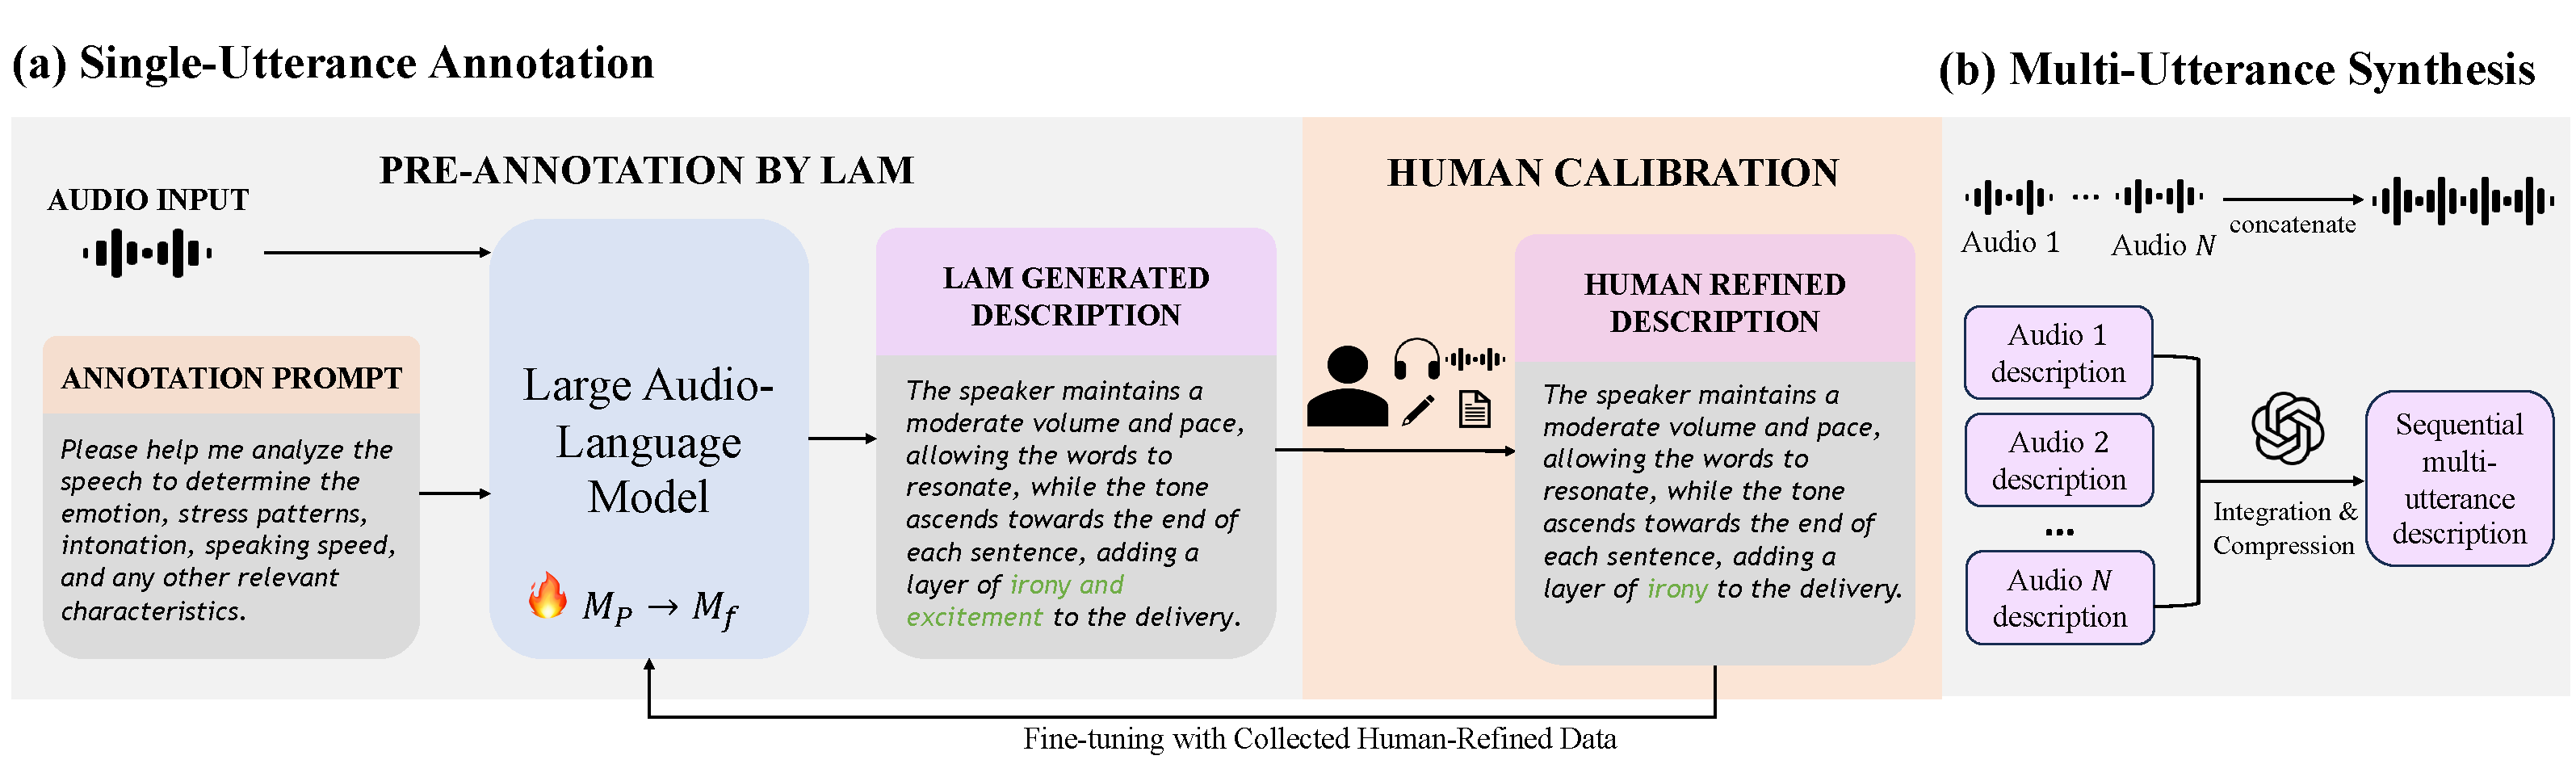
\includegraphics[width=\linewidth]{figs/data_annotation.pdf}
  \caption{Overview of the DramaPara annotation and synthesis pipeline. (a) \textbf{Single-Utterance Annotation} employs a human-in-the-loop strategy: a Large Audio-Language Model generates pre-annotations based on the audio and prompts, which are then rigorously calibrated by human experts to eliminate inaccuracies (e.g., hallucinated emotions). The collected human-refined data is iteratively used to fine-tune the pretrained model ($M_p$) into a fine-tuned version ($M_f$) to enhance future pre-annotation quality. (b) \textbf{Multi-Utterance Synthesis} constructs sequential multi-utterance data by first concatenating $N$ adjacent single-utterance audio clips. Concurrently, their corresponding calibrated descriptions are integrated and compressed by an LLM to form a cohesive narrative, effectively capturing the chronological and dynamic paralinguistic evolution across continuous conversational turns.}
  \label{fig:annotation_pipeline}
\vspace{-0.2cm}
\end{figure*}

\textbf{Data Source:} To closely approximate real-world acoustic complexity and highly expressive emotional nuances, the source audio is extracted from classic American TV dramas. These recordings naturally contain rich paralinguistic information intertwined with overlapping background noise, ambient sound effects, and dynamic scene transitions. All audio clips are utilized in strict accordance with the principles of fair use, and the dataset is intended solely for non-commercial academic research purposes.

\textbf{Single-Utterance Human-in-the-Loop Annotation:} The raw audio tracks are first segmented into utterance-level clips using Voice Activity Detection (VAD)~\cite{Silero_VAD}. We then implement a highly efficient human-in-the-loop annotation pipeline, as illustrated in Figure~\ref{fig:annotation_pipeline}(a). Initially, an off-the-shelf LAM is deployed to generate pre-annotations for the segmented clips\footnote{We use SALMONN-13B for pre-annotations. The checkpoint could be found on \url{https://huggingface.co/tsinghua-ee/SALMONN}.}. Professional human annotators then rigorously review and calibrate these descriptions to ensure accuracy. Notably, to optimize annotation efficiency, we adopted a batched iterative strategy: after accumulating approximately 50 hours of human-calibrated data, we fine-tuned the pre-annotation LAM using this high-quality subset. Annotator feedback confirmed that this intermediate fine-tuning significantly reduced the error rate of the pre-annotations, drastically decreasing the manual modification workload for the remainder of the dataset.

\textbf{Multi-Utterance Sequential Synthesis:} The multi-utterance data is constructed subsequently based on the single-utterance dataset. As depicted in Figure~\ref{fig:annotation_pipeline}(b), we concatenate $N$ ($N \in [3, 5]$) adjacent single-utterance audio clips into a continuous multi-utterance audio sequence, while systematically integrating their corresponding calibrated single-utterance labels. It is worth noting that, as reported in Table~\ref{tab:statistics}, the total duration of the multi-utterance dataset is lower than that of the single-utterance dataset. This discrepancy primarily arises from a strict duration-based filtering process. Because excessively long audio sequences significantly increase the task difficulty for the models, we filter out any concatenated multi-utterance audio that exceeds 30 seconds in total duration. Finally, a Large Language Model (LLM) is prompted to transform the discrete single-utterance descriptions into a cohesive, chronological narrative. Because the initial LLM outputs tend to be overly verbose, we employ a secondary LLM compression and refinement pass to distill the vocabulary, ensuring the final sequential descriptions are concise, accurate, and contextually fluent\footnote{GPT-4o-mini is used for transforming and refinement, the specified version is \texttt{gpt-4o-mini-2024-07-18}.}.

\section{Experimental Setup}
\label{sec:experiments}

\begin{figure*}[t]
  \centering
  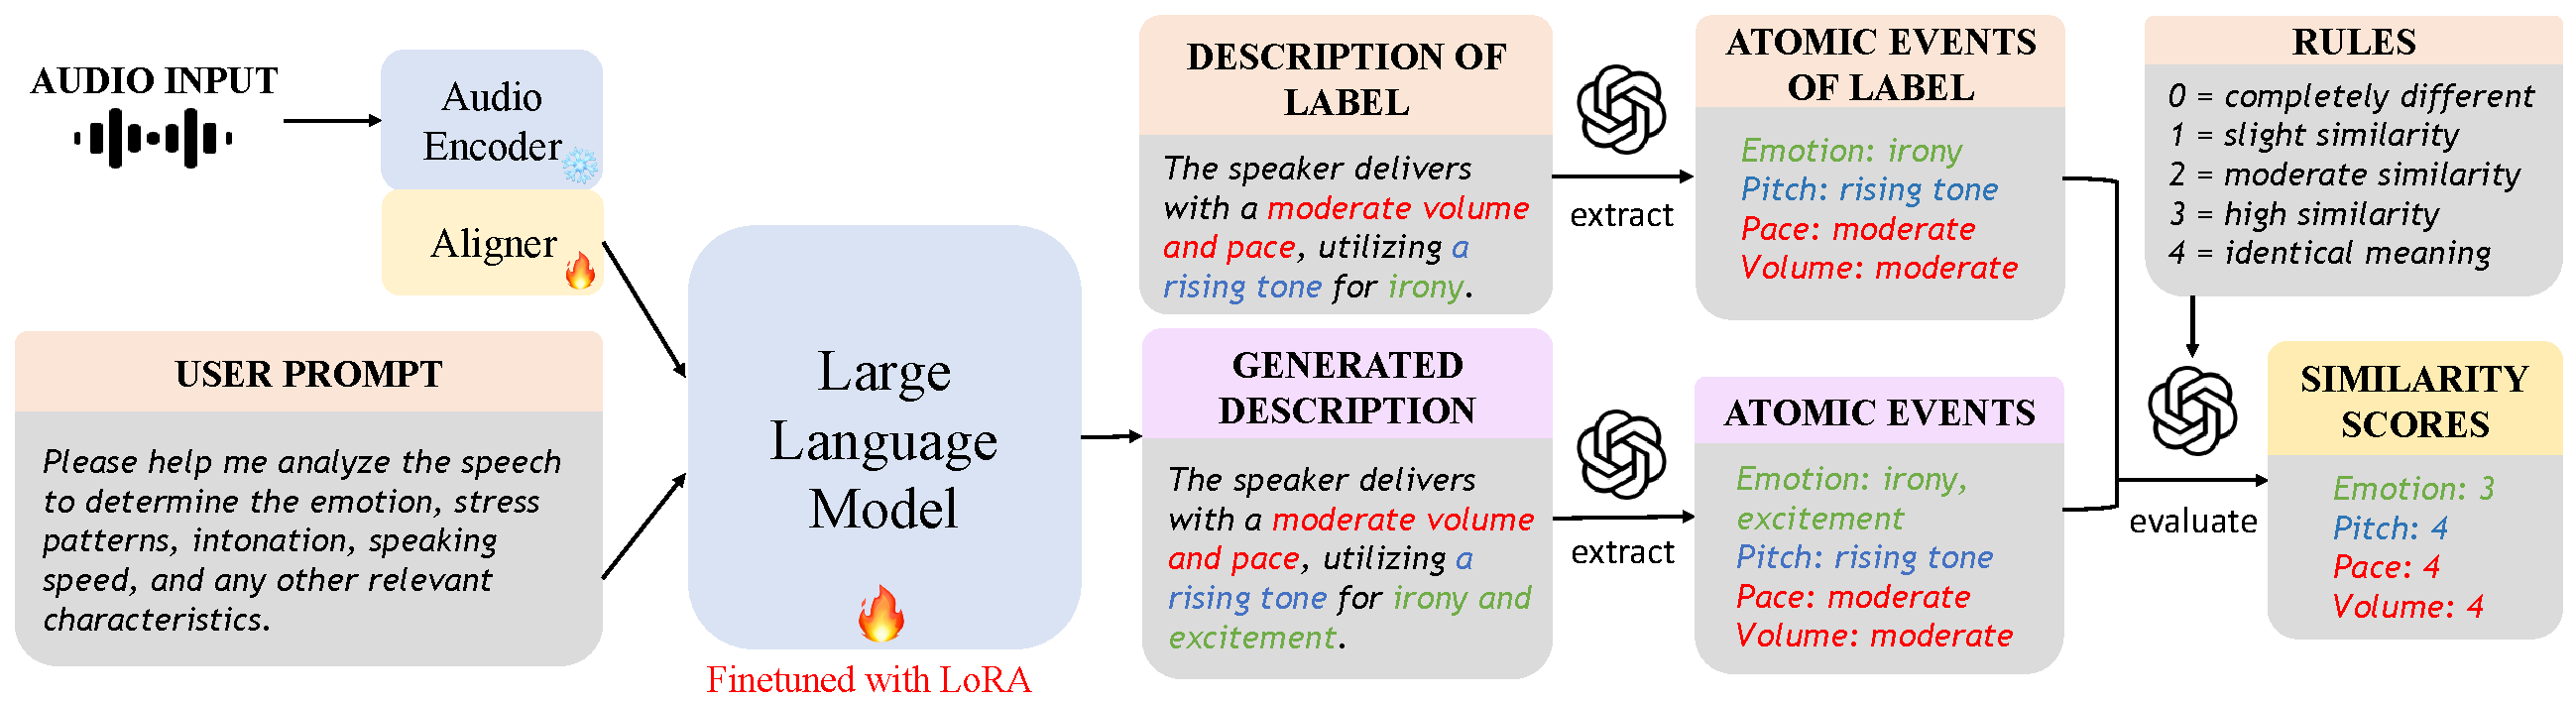
\includegraphics[width=\linewidth]{figs/infer_eval.pdf}
  \caption{Illustration of the inference and LLM-as-a-Judge evaluation pipeline. During inference, the audio and user prompt are processed by the LAM (with LoRA fine-tuning applied to the aligner and LLM) to generate a paralinguistic description. For evaluation, an advanced LLM extracts atomic events (e.g., emotion, pitch, pace, volume) from both the generated description and the ground-truth label. An LLM evaluator then compares these aligned events, assigning similarity scores on a discrete scale from 0 to 4.}
  \label{fig:infer_eval}
\vspace{-0.2cm}
\end{figure*}

\begin{table*}[th]
  \caption{Evaluation results of paralinguistic description capabilities (scored from 0 to 4) on the 5-hour test set. The best results for each base model are highlighted in \textbf{bold}.}
  \label{tab:main_results}
  \centering
  % \resizebox{\textwidth}{!}{
  \begin{tabular}{l cccc c cccc}
    \toprule
    \multirow{2}{*}{\textbf{Model Configuration}} & \multicolumn{4}{c}{\textbf{Single-Utterance Task}} && \multicolumn{4}{c}{\textbf{Multi-Utterance Sequential Task}} \\
    \cmidrule{2-5} \cmidrule{7-10}
    & Emotion & Pace & Pitch & Volume && Emotion & Pace & Pitch & Volume \\
    \midrule
    Qwen2.5-Omni (Zero-shot) & 0.74 & 2.02 & 1.41 & \textbf{2.43} && 0.99 & 1.29 & 1.26 & 1.12 \\
    \quad + SFT (DramaPara) & \textbf{0.99} & \textbf{2.40} & \textbf{2.45} & 2.33 && \textbf{1.46} & \textbf{1.55} & \textbf{1.48} & \textbf{1.35} \\
    \midrule
    SALMONN (Zero-shot) & 1.45 & 2.74 & 2.32 & 2.31 && 1.09 & 1.21 & 1.10 & 1.04 \\
    \quad + SFT (DramaPara) & 1.52 & 2.73 & 2.44 & 3.58 && 1.60 & \textbf{1.60} & \textbf{1.70} & \textbf{1.81} \\
    \quad + SFT + DPO & \textbf{1.56} & \textbf{2.75} & \textbf{2.55} & \textbf{3.60} && \textbf{1.64} & 1.52 & 1.66 & 1.73 \\
    \bottomrule
  \end{tabular}
  % }
\vspace{-0.3cm}
\end{table*}

\subsection{Data Configuration}
To evaluate the models, we partition the DramaPara dataset into training and testing sets. From the $\sim$492 hours of single-utterance data, we randomly sample approximately 5 hours for testing, utilizing the remaining 487 hours for training. To strictly prevent data leakage, the multi-utterance training and testing sets are synthesized exclusively from their corresponding single-utterance splits. During training, we adopt a mixed-task strategy, shuffling both single- and multi-utterance data to equip the models with both isolated profiling and sequential reasoning capabilities.

\subsection{Supervised Fine-Tuning (SFT)}
We perform SFT on two representative open-source LAMs: SALMONN\footnote{\url{https://huggingface.co/tsinghua-ee/SALMONN}}~\cite{tangsalmonn} and Qwen2.5-Omni\footnote{\url{https://huggingface.co/Qwen/Qwen2.5-Omni-7B}}~\cite{Qwen2.5-Omni}. For both models, we freeze the audio encoder and fine-tune the cross-modal aligner alongside the LLM. The LLM is fine-tuned using Low-Rank Adaptation (LoRA)~\cite{hu2022lora} with $r=8$ and $\alpha=32$.

Training is conducted over 10 epochs using a cosine learning rate scheduler with a peak learning rate of $3 \times 10^{-6}$ and a 5\% warmup ratio. To ensure a fair comparison, both models maintain an effective total batch size of 24. Specifically, SALMONN is fine-tuned using its official codebase\footnote{\url{https://github.com/bytedance/SALMONN}} on 8 NVIDIA H20 GPUs (batch size of 3 per GPU), while Qwen2.5-Omni is fine-tuned via the \texttt{ms-swift} framework\footnote{\url{https://github.com/modelscope/ms-swift}}~\cite{zhao2024swift} on a single H20 GPU (batch size of 24).

\subsection{Reinforcement Learning via DPO}
To further align the model's paralinguistic perception with human preferences, particularly for complex emotional states, we apply Direct Preference Optimization (DPO)~\cite{dpo} to the SFT-tuned SALMONN model. DPO optimizes the policy model $\pi_\theta$ against a reference model $\pi_{\text{ref}}$ by directly maximizing the log-likelihood of the preferred response $y_w$ over the rejected response $y_l$, avoiding the need for an explicit reward model. The loss is formulated as:
$$ 
\begin{aligned}
\mathcal{L}_{\text{DPO}} = -\mathbb{E}_{(x, y_w, y_l)\sim \mathcal{D}} \bigg[ \log \sigma \bigg( &\beta \log \frac{\pi_\theta(y_w|x)}{\pi_{\text{ref}}(y_w|x)} \\
&- \beta \log \frac{\pi_\theta(y_l|x)}{\pi_{\text{ref}}(y_l|x)} \bigg) \bigg] 
\end{aligned}
$$
where $x$ is the input (audio and prompt), $\sigma$ is the sigmoid function, and $\beta$ controls the divergence from the reference model.

To construct the preference dataset $\mathcal{D}$, we randomly sample 2,000 single-utterance and 1,000 multi-utterance instances from the training set. For each instance, we generate 5 responses using different random seeds. To evaluate the quality of these responses, we employ the LLM-as-a-Judge methodology detailed in Section~\ref{subsec:eval} to obtain dimension-specific similarity scores against the ground-truth labels. Given that emotion recognition is significantly more challenging than other acoustic features, we compute a final composite score using a weighted mechanism: the Emotion score carries a weight of 1.0, while the Volume, Pitch, and Pace scores each carry a weight of 0.1. We rank the 5 responses based on this composite score, selecting the highest-scoring response as $y_w$ and the lowest as $y_l$. Finally, to ensure high-quality contrastive signals, we strictly filter the pairs, retaining only the top 20\% with the largest score margins for the DPO mixed training.

For the DPO training configuration, we train the model for 1 epoch with a learning rate of $5.0 \times 10^{-7}$. The DPO-specific hyperparameters are set to $\beta = 0.1$ and a label smoothing factor of $0$. The training is executed on 8 NVIDIA H20 GPUs, utilizing a micro-batch size of 1 per GPU.

\subsection{Evaluation Methodology}
\label{subsec:eval}
As illustrated in Figure~\ref{fig:infer_eval}, we adopt an LLM-as-a-Judge paradigm for automatic evaluation. First, an advanced LLM\footnote{GPT-4o-mini is used for automated evaluation, the specified version is  \texttt{gpt-4o-mini-2024-07-18}.} extracts atomic paralinguistic events (emotion, volume, pitch, pace) from both the model's generated narrative and the ground-truth human label. The LLM then acts as a strict evaluator, systematically comparing the generated atomic events against the ground truth. Following a carefully designed prompt, the LLM assigns a similarity score ranging from 0 to 4 for each dimension, where a higher score indicates greater alignment with the human-calibrated reference.

\section{Results and Analysis}
\label{sec:results}

The overall experimental results, evaluated on the 5-hour hold-out test set using the 0-4 LLM-as-a-Judge metric, are presented in Table~\ref{tab:main_results}. The findings clearly validate the necessity of the DramaPara dataset and the effectiveness of our mixed training strategy.

\textbf{Baseline Limitations in Complex Scenarios:} 
Both the pre-trained SALMONN and Qwen2.5-Omni models exhibit sub-optimal performance in their zero-shot states. Furthermore, their performance degrades drastically on the Multi-Utterance Sequential Task. This substantial degradation confirms our hypothesis that existing LAMs trained on clean, isolated audio lack the sequential reasoning capabilities required to track dynamic paralinguistic evolution in real-world conversational turns.

\textbf{Significant Gains via SFT:} 
Fine-tuning the models on the DramaPara dataset yields substantial improvements across the board. For Qwen2.5-Omni, pitch and emotion perception in the single-utterance task increased significantly (e.g., pitch from 1.41 to 2.45). For SALMONN, the SFT model dramatically boosts volume perception (from 2.31 to 3.58) and restores its reasoning ability in the sequential task, with average scores jumping by over 45\% relatively compared to the zero-shot baseline. The robust gains across both architectures demonstrate that DramaPara successfully provides high-quality alignment signals for complex acoustic environments.

\textbf{Effectiveness of RL via DPO:}
As detailed in Section~\ref{sec:experiments}, we applied DPO to the SALMONN model with a specific emphasis on emotion accuracy (assigning a reward weight of 1.0 to Emotion vs. 0.1 to other dimensions). The results strongly align with our design objective: the DPO-tuned model achieves the highest Emotion scores in both the single-utterance (1.56) and multi-utterance (1.64) tasks. 

While DPO brings consistent, albeit slight, enhancements to pitch and volume on the single-utterance task, we observe minor score fluctuations in the multi-utterance pace and pitch metrics. This is an expected trade-off in reinforcement learning; by heavily anchoring the preference optimization towards solving the highly challenging emotion dimension, the model slightly compromises its focus on simpler acoustic attributes. Nevertheless, the DPO strategy proves highly effective in aligning the model's complex emotional perception with human expectations in naturalistic scenarios.

\section{Conclusion}
\label{sec:conclusion}

In this work, we introduced \textbf{DramaPara}, a comprehensive dataset extracted from TV dramas designed to bridge the domain gap in paralinguistic understanding within complex acoustic environments. By establishing both single-utterance isolated profiling and multi-utterance sequential tasks, and applying a mixed training strategy involving SFT and DPO, we significantly enhanced the capability of existing LAMs to decode fine-grained and dynamically evolving human expressions. Furthermore, DramaPara paves a scalable path for auto-annotating massive unlabeled drama data and provides a crucial foundation for training highly controllable, expressive Text-to-Speech (TTS) systems.

% {\color{blue}
\section{Generative AI Use Disclosure}
% The extent of Generative AI use must be disclosed. This section may be in the 5th or 6th pages of regular papers, or the 9th or 10th pages of long papers.  ISCA policy says: \textit{All (co-)authors must be responsible and accountable for the work and content of the paper, and they must consent to its submission. Any generative AI tools cannot be a co-author of the paper. They can be used for editing and polishing manuscripts, but should not be used for producing a significant part of the manuscript}.
In this work, Large Language Models (LLMs) were utilized across three key stages. For data annotation, LLMs generated initial paralinguistic pre-annotations and synthesized multi-utterance narratives, significantly accelerating our human-in-the-loop pipeline. During model evaluation, we employed an LLM-as-a-Judge paradigm to extract atomic acoustic events and objectively score the generated descriptions against ground-truth labels. Additionally, LLMs were used to polish the language and improve the structural clarity of this manuscript.
% }



\bibliographystyle{IEEEtran}
\bibliography{mybib}

\end{document}

%%% Local Variables:
%%% mode: LaTeX
%%% TeX-master: t
%%% End:
